\documentclass[brudnopis]{xmgr}
% Jeśli nowe rozdziały mają się zaczynać na stronach
% nieparzystych:
%\documentclass[openright]{xmgr}

\usepackage{epigraph}
\usepackage{url}
\usepackage{float}

\defaultfontfeatures{Scale=MatchLowercase}
\setmainfont[Numbers=OldStyle,Ligatures=TeX]{Minion Pro}
\setsansfont[Numbers=OldStyle,Ligatures=TeX]{Myriad Pro}
% for fontspec version < 2.0
%\setmainfont[Numbers=OldStyle,Mapping=tex-text]{Minion Pro}
\setsansfont[Numbers=OldStyle,Mapping=tex-text]{Myriad Pro}
%\setmonofont[Scale=0.75]{Monaco}

% Opcjonalnie identyfikator dokumentu
% drukowany tylko z włączoną opcją 'brudnopis':
\wersja   {wersja wstępna [\ymdtoday]}

\author   {Piotr Lewandowski}
\nralbumu {215575}
\email    {poczta@piotrl.net}

\title    {Analiza wpływu nawyków muzycznych na aktywności wykonywane przy komputerze}
\date     {2017}
\miejsce  {Gdańsk}

\opiekun  {dr W. Bzyl}

% dodatkowe polecenia
%\renewcommand{\filename}[1]{\texttt{#1}}
%\definecolor{stress}{cmyk}{0,1,0.13,0} % RubineRed
%\definecolor{topic}{cmyk}{0.98,0.13,0,0.43} % MidnightBlue

\begin{document}

% streszczenie
\begin{abstract}
    W ramach pracy magisterskiej napisano aplikację internetową,
    wdrożoną w chmurze Digital Ocean pod adresem http://tbd.digitalocean.com/
    z przygotowanymi danymi testowymi pod kontem (user: test, login: test).

    Aplikacja umożliwia agregację danych użytkownika z dwóch serwisów,
    RescueTime — lista aktywności oraz
    Last.fm — lista odsłuchiwanych utworów.
    Pobrane dane są połączone na wspólnej osi czasu i wizualizowane pod różnymi względami za pomocą wykresów oraz tabel.

    Mechanizm agregacji napisany jest w języku Java i frameworku Spring,
    dane przechowywane są w bazie danych PostgreSQL,
    a warstwa wizualna została stworzona w JavaScript
    z użyciem biblioteki generującej wykresy — C3.js
    oraz frameworka Material Design.

    Kod znajduje się w prywatnym repozytorium GIT (pod adresem \url{https://github.com/piotrl/master-thesis}),
    pytania o dostęp lub o pracę można kierować na mail: poczta@piotrl.net.
\end{abstract}

% słowa kluczowe
\keywords{
    Aggregation,
    Data Integration,
    Data Visualisation,
    PostgreSQL,
    JavaScript,
    Java
}

% tytuł i spis treści
\maketitle

% wstęp
\introduction

\epigraph{Without deviation from the norm, progress is not possible}{\textit{Frank Zappa}}

[Work in progress]

Podczas pracy często słucham muzyki, by się odciąć od zewnętrznych dźwięków oraz odpowiednio nastroić.
Spotyka się na artykuły twierdzące, że odpowiednio dobrana muzyka wpływa na lepszą koncentrację.
Popularnym przykładem jest wystąpienie Willa Henshalla na konferencji TEDx,
którą w momencie pisania pracy obejrzano ponad 400 tysięcy razy:

Jednym z pytań w corocznej sondzie serwisu StackOverflow jest pytanie o muzyczne preferencje podczas programowania.
Na to pytanie odpowiedziało ponad 36 tysięcy osób \cite{stackoverflow:survey2017}.

\begin{figure}
  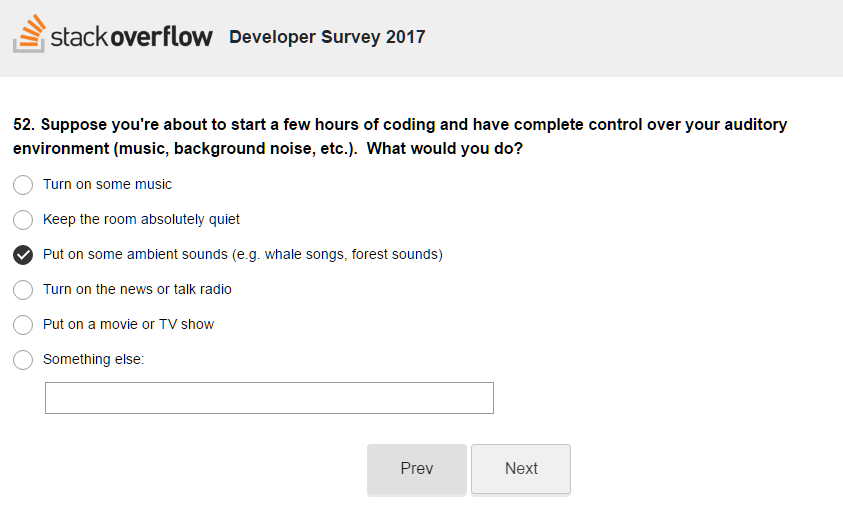
\includegraphics[width=\linewidth]{fig/stack_overflow_music.png}
  \caption{Pytanie o preferncje muzyczne na StackOverflow}
  \label{fig:Pytanie o preferncje muzyczne na StackOverflow}
\end{figure}

\chapter{Import danych}

    \section{Wybór dostawców danych}

    Podstawą działania aplikacji są dane z komputera użytkownika,
    lista aktywności wykonywanych w danej jednostce czasu oraz odsłuchiwana muzyka.
    Aby zdobyć te dane, postanowiłem nie pisać programu śledzącego procesy (daemon),
    lecz skorzystać z istniejących serwisów, z których użytkownicy mogli już korzystać.

    Przy wyborze rozwiązania zależało mi na tym, by serwisy były już dłuższy czas na rynku
    oraz udostępniały archiwalne dane za pomocą publicznego API.
    Dzięki temu nie ma potrzeby oczekiwania na zbudowanie zioru danych do analizy po rejestracji nowego użytkowniku,
    od razu można przeanalizować dane z okresu sprzed rejestracji.

    Zdecydowałem się skorzystać z dwóch dobrze znanych mi serwisów - RescueTime oraz last.fm,
    oba serwisy są najpopularniejsze w swojej klasie oraz dostarczają publiczne API dla danych użytkownika.

        \section*{RescueTime}

%        \begin{figure}
%          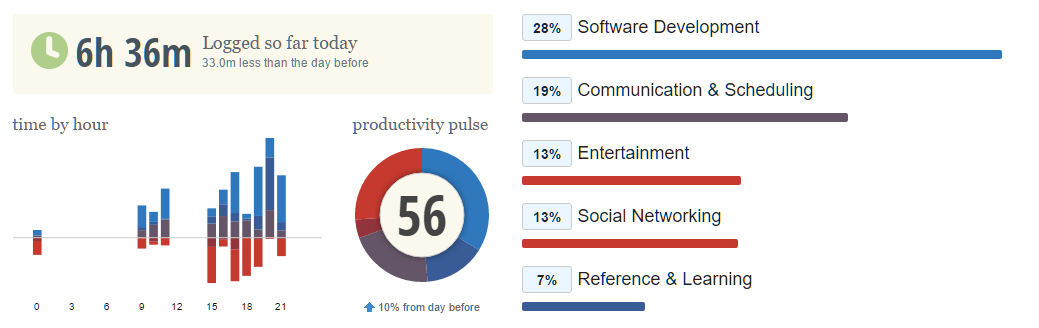
\includegraphics[width=\linewidth]{fig/rescuetime-daily-dashboard.png}
%          \caption{Codzienny raport aktywności RescueTime}
%          \label{fig:RescueTime}
%        \end{figure}

        RescueTime to program, który loguje aktualnie otwarte okna
        i raz na minutę wysyła te dane do serwisu internetowego RescueTime.com.
        Podstawową cechą tego serwisu jest automatyczne kategoryzowanie aktywności oraz ustawienie produktywności w 5 punktowej skali:
        „Bardzo produktywny”, „Produktywny”, „Neutralny”, „Rozpraszający” i „Bardzo rozpraszający”.

        Serwis uczy się doasowywać aktywności do kategorii na podstawie wcześniejszych oznaczeć użytkowników.
        Dla przykładu odtwarzacz wideo VLC jest przypisany do kategorii „Entertainment” ze statusem „Bardzo rozpraszający”,
        natomiast przeglądanie plików programem Windows Explorer jest w kategorii „Utilities” ze statusem „Neutralny”.

        Dzięki temu jesteśmy w stanie obliczyć nasz codzienny współczynnik produktywności,
        sumując czas spędzony na aktywnościach z każdej kategorii.

        \begin{table}[]
        \centering
        \begin{tabular}{lll}
        \hline
        \multicolumn{1}{l|}{Aktywność} & \multicolumn{1}{l|}{Kategoria} & Produktywność \\ \hline
        idea64                         & Software Development           & +2            \\
        NotePad++                      & Software Development           & +2            \\
        postgresql.org                 & Reference \& Learning          & 0             \\
        twitter.com                    & Social Networking              & -1            \\
        analytics.twitter.com          & Social Networking              & -2            \\
        youtube.com                    & Entertainment                  & -2            \\
        outlook.office.com             & Communication \& Scheduling    & 0             \\
        wunderlist                     & Business                       & +2
        \end{tabular}
        \caption{
            Lista przykładowych aktywności wraz z ich kategoriami. Skala produktywności od +2 do -2
            \newline Źródło: Opracowanie własne.
        }
        \label{RescueTime - lista przykładowych aktywności}
        \end{table}

        Program jest w stanie rozpoznać nie tylko tytuły aktualnie otwartych okien,
        ale również w przypadku przeglądarki – adresy odwiedzanych stron internetowych,
        jest to bardzo ważne ze względu na dominującą ilość czasu spędzonego w samej przeglądarce.

        Dostęp do informacji użytkownika odbywa się po REST API z tokenem uwierzytelniającym,
        który użytkownik musi wygenerować na stronie RescueTime.com.
        Po poprawnym uwierzytelnieniu, mamy dostęp do danych sprzed 3 miesięcy w formacie JSON.

        \section*{last.fm}

        Last.fm to serwis społecznościowy dla fanów muzyki,
        pomagający odkrywać nowych artystów na podstawie historii użytkownika.

        Wtyczka "last.fm Scrobbler"\cite{lastfm:trackmymusic} integruje się z wieloma odtwarzaczami muzycznymi, np. Spotify.
        Każdy odsłuchany w co najmniej w połowie utwór jest logowany do bazy danych,
        w której na podstawie meta-tagów jest przypisywany do artysty, płyty oraz gatunku muzycznego.

		 Last.fm udostępnia szereg metod REST API \cite{lastfm:apidoc}, 
		 dla mnie szczególnie istotne są te związane z odtworzeniami użytkownika oraz szczegółowych informacji o piosenkach i artystach.

       Metoda user.getRecentTracks % TODO


		% identyfikuje swoje dane za pomocą MBID \cite{lastfm:mbid}

        \begin{figure}
          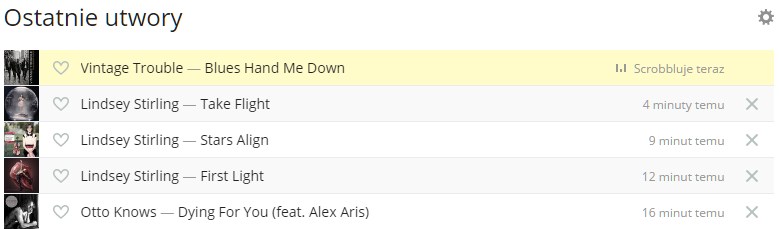
\includegraphics[width=\linewidth]{fig/lastfm-now-listening.png}
          \caption{Raport słuchanej muzyki w last.fm}
          \label{fig:Last.fm}
        \end{figure}

        \section*{Komunikacja z zewnętrznymi serwisami}
			TODO

    \section{Mechanizm importu danych}

        Oba z wymienionych serwisów udostępniają część danych, które użytkownik zgromadził na swoim koncie.
        Dostęp ten jest realizowany przez API, po okazaniu odpowiednich tokenów uwierzytelniających, mamy dostęp do danych użytkownika.

        Przed analizą, konieczne jest pobranie danych do własnej bazy danych oraz stworzenie modelu relacji pomiędzy nimi.
        Proces pobierania nazywam agregacją danych lub importem danych i jest on podstawą działania aplikacji,
        ponieważ to w nim zdobywamy interesujące nas informacje wykorzystywane do późniejszych obliczeń.

        Aby aplikacja nie była jednorazowego użytku, wraz z upływem czasu należy dla każdego użytkownika dostarczać
		  kolejne porcje danych z zewnętrznych serwisów.
        Rodzi to szereg problemów oraz wyznacza pewne cechy, które napisany mechanizm musi spełniać.

        \subsection*{Niezależność}
        Podczas pobierania danych dla jednego użytkownika może wystąpić błąd, np. poprzez tymczasową niedostępność API,
        nie powinien on wpłynąć na agregacje innych użytkowników, ani na działanie mechanizmu w przyszłości dla tego samego użytkownika.
		 
  		 Części błędów można się spodziewać, np. lastfm udostępnia do każdej metody API listę błędów które może zwrócić zamiast odpowiedzi.
		 Z drugiej strony, mogą wystąpić błędy po naszej stronie - zwłaszcza gdy API nie jest bardzo dobrze udokumentowane 
		 lub nie mamy zbyt dużego doświadczenia z pracy z nimi, np. podczas mapowania odpowiedzi na obiekty lub przy zapisie danych do bazy.

		 Można sobie z tym radzić na kilka sposobów, przechwytując wyjątki podczas wysyłania każdego requestu oraz budując globalny error handler.


        \subsection*{Ciągłość}
        Celem codzienne uruchamianie procedury i pobranie najnowszych lub brakujących danych do systemu,
        API pozwalają nam na wybranie tylko małego fragmentu danych, istotne jest więc by zacząć import
        od momentu ostatniego poprawnie wczytanego rekordu dla danego użytkownika.

        \subsection*{Powtarzalność}

    \section{Powszechne problemy przy komunikacji z API}

        \subsection*{Ograniczenia dostawcy API}

        \subsection*{Autoryzacja}

        \subsection*{Braki dostępu}

        \subsection*{Zepsute dane}
        API nie gwarantuje istnienia ani poprawności wszystkich informacji.
        Przykładowo last.fm do identyfikacji utworu dostarcza jego identyfikator i pełną nazwę.
        Zawsze bezpieczniej jest korzystać z identyfikatora, ponieważ w nazwie mogą występować niebezpieczne dane np. znaki UTF-8,
        jednak istnieją, rekordy dla których identyfikator jest pusty. \cite{Goldfarb:2002:CFG}

        \subsection*{Wydajność}
        Dobrze jest kopiować wszystkie powtarzalne informacje do własnej bazy danych,
        dzięki temu możemy ograniczyć ilość żądań do API, które może mieć limity.

\chapter{Analiza danych}

    \section{Opis zebranych danych}

    \section{Data fusion - Łączenie danych w czasie}

        \subsection*{Korekta}

        \subsection*{Integracja dwóch źródeł danych}

     \section{Budowa raportów na podstawie szeregów czasowych}

\chapter{Wizualizacja danych}

     \section{Jeden zbiór danych - wiele interpretacji}

     \section{Wybór odpowiednich metod wizualizacji danych}

     \section{Analiza danych z punktu widzenia użytkownika}

\chapter{Architektura}

\section{Wydajnosc aplikacji}

\section{Testy jednostkowe}

\section{Narzędzia}


% zakończenie
\summary
[Work in progress]

% literatura (obowiązkowo):
\bibliographystyle{unsrt}
\bibliography{xml}

% spis tabel (jeżeli jest potrzebny):
\listoftables

% spis rysunków (jeżeli jest potrzebny):
\listoffigures

\oswiadczenie

\end{document}
